%KECReportFormat.tex
%%%%%%%%%%%%%%%%%%%%%%%%%%%%%%%%%%%%%%%%%%%%%%%%%%%%%%%%%%%%%%%%%%%%%%%%%%%
%DO NOT MAKE CHANGES IN THIS FILE

\documentclass[12pt, a4paper]{report}
\usepackage[left = 1.5in, right = 1in, top = 1in, bottom = 1in]{geometry}%for margin
\usepackage{amsfonts, amsmath, amssymb} %for mathematical equations
\usepackage{graphicx} %for images
\usepackage{times} %font Times New Roman Font
\usepackage{float} %required if you use H(strictly here) position for floats
\usepackage[skip = 8pt,tableposition=top, figureposition=bottom]{caption}%adjust spacing of captions and specify where captions are
\usepackage{hyperref} % for easy Navigation in document, also puts links in TOC, LOF, LOT...
\usepackage{setspace} %to change line spacing in some portion \singlespacing \onehalfspacing \doublespacing
\usepackage{acro} %for List of Abbrreviation and Symbol
\acsetup{first-style = short} % set to display only short form on the command \ac{}

%packages required for complex tables
\usepackage{bigstrut} 
\usepackage{multirow}

\renewcommand{\contentsname}{Table of Contents} %Change TOC Heading ... default is "Contents" 

\parindent 0pt	%removes the indent in paragraph
\setlength{\parskip}{18pt}	%for paragraph spacing
\renewcommand{\baselinestretch}{1.5}   %Line Spacing = 1.5 line-spaces

%to reduce spacing in sections
\usepackage{titlesec}
\titlespacing*{\section}{0pt}{0pt}{0pt} %left, top, bottom spacings
\titlespacing*{\subsection}{0pt}{0pt}{0pt}
\titlespacing*{\subsubsection}{0pt}{0pt}{0pt}
\titlespacing*{\paragraph}{0pt}{0pt}{0pt}
\titlespacing*{\subparagraph}{0pt}{0pt}{0pt}

%adjust fontsizes\ of sections
\titleformat*{\section}{\fontsize{14pt}{18pt}\bfseries}
\titleformat*{\subsection}{\fontsize{13pt}{18pt}\bfseries}
\titleformat*{\subsubsection}{\fontsize{12pt}{18pt}\bfseries}
\titleformat*{\paragraph}{\fontsize{12pt}{18pt}\bfseries}
\titleformat*{\subparagraph}{\fontsize{12pt}{18pt}\bfseries}

%to reduce separation between points in list
\usepackage{enumitem}
\setlist[enumerate]{nosep} % no separation between items in enumerate
\setlist[itemize]{nosep} % no separation between items in itemize
%use \vspace{-18pt} before list to reduce paragraph spacing between list and preceeding paragraph.

%Changes for Chapter Heading Spacing and formats for numbered chapters
\makeatletter
\def\@makechapterhead#1{%
  %\vspace*{50pt}%
  {  \MakeUppercase{\ifnum \c@secnumdepth >\m@ne
        \fontsize{16pt}{1}\bfseries \@chapapp \space \thechapter\vspace{5pt}\\
    \fi
    \interlinepenalty\@M
     \bfseries #1}\par\nobreak
    %\vskip 0pt
  }}
\makeatother

%%%%%%%%%%%%%%%%%%%%%%%%%%%%%%%%%%%%%%%%%%%%%%%%%%%%%%%%%%%
%to adjust Heading spacings and fonts For unnumbered chapters, TOC, LOF ...
\makeatletter
% Redefine the \chapter* header macro to remove vertical space
\def\@makeschapterhead#1{%
  %\vspace*{50\p@}% Remove the vertical space
  {\newpage \parindent \z@ \raggedright
    \normalfont
    \interlinepenalty\@M
    \center \fontsize{16pt}{1} \bfseries \MakeUppercase{#1}\par\nobreak
    %\vskip 18\p@ % adjust space after heading 18pt
  }}
\makeatother 
%%%%%%%%%%%%%%%%%%%%%%%%%%%%%%%%%%%%%%%%%%%%%%%%%%%%%%%%%%%

%%%%%%%%%%%%%%%%%%%%%%%%%%%%%%%%%%%%%%%%%%%%%%%%%%%%%%%%%%%%%%%%%%%%%%%%%%%
% newcommand for generating Cover Page
\newcommand{\KECcoverpage}
{
\begin{titlepage}
\begin{center}
\Large{\textbf{KANTIPUR ENGINEERING COLLEGE}}\\
\large{\textbf{(Affiliated to Tribhuvan University)}}\\
\large{\textbf{Dhapakhel, Lalitpur}}\\
\vfill	%vertically fill the space 
\begin{figure}[h] % h: put logo "here"
\begin{center}
\includegraphics[width=25mm, height = 25mm]{images/logo.png}
\end{center}
\end{figure}

\large{\textbf{[Subject Code: \subCode]}}\\ %Change This Line
\large{\textbf{A \MakeUppercase{\project} \MakeUppercase{\doc} ON}}\\ %Change This Line
\Large{\textbf{\MakeUppercase{\projectTitle}}}\\

\vfill	%vertically fill the space 
\large{\textbf{Submitted by:}}\\
\large{\textbf{\submittedBy}}\\
\vfill	%vertically fill the space 
\textbf{A \MakeUppercase{\project} SUBMITTED IN PARTIAL FULFILLMENT OF THE REQUIREMENT FOR THE DEGREE OF \MakeUppercase{\degree}}\\

\vfill	%vertically fill the space 
\large{\textbf{Submitted to:}}\\
\large{\textbf{\submittedTo}}\\
\vfill
\large{\textbf{\defMonth, \defYear}}
\pagebreak
\end{center}
\end{titlepage}
}
%%%%%%%%%%%%%%%%%%%%%%%%%%%%%%%%%%%%%%%%%%%%%%%%%%%%%%%%%%%%%%%%%%%%%%%
% newcommand for generating Cover Page
%Title Page
\newcommand{\KECtitlepage}
{
\begin{titlepage}
\begin{center}
\Large{\textbf{\MakeUppercase{\projectTitle}}}\\

\vfill	%vertically fill the space 

\large{\textbf{Submitted by:}}\\
\large{\textbf{\submittedBy}}\\


\ifhassupervisor % Displays Supervisor name only if \hassupervisortrue
	\vfill	%vertically fill the space 
	\large{\textbf{Supervised by:}}\\
	\large{\textbf{\supervisor}}\\
	\large{\textbf{\degSup}}\\
\fi

\vfill	%vertically fill the space 
\textbf{A \MakeUppercase{\project} SUBMITTED IN PARTIAL FULFILLMENT OF THE REQUIREMENT FOR THE DEGREE OF \MakeUppercase{\degree}}\\

\vfill	%vertically fill the space 
\large{\textbf{Submitted to:}}\\
\large{\textbf{\submittedTo}}\\
\large{\textbf{Kantipur Engineering College}}\\
\large{\textbf{Dhapakhel, Lalitpur}}\\

\vfill
\large{\textbf{\defMonth, \defYear}}
\thispagestyle{empty}\\ %to remove page number
\pagebreak
\end{center}
\end{titlepage}
}
%%%%%%%%%%%%%%%%%%%%%%%%%%%%%%%%%%%%%%%%%%%%%%%%%%%%%%%%%%%%%%%%%%%%%%
%command for copyright page
\newcommand{\KECcopyright}
{
\chapter*{Copyright}%Required only for Final Defense of Major Project
\addcontentsline{toc}{chapter}{Copyright}
The author has agreed that the library, Kantipur Engineering Collage, may make this report freely available for inspection. Moreover the author has agreed that permission for extensive copying of this report for scholarly purpose may be granted by the supervisor(s), who supervised the project work recorded herein or, in their absence, by the Head of the Department wherein this project was done. It is understood that due recognition will be given to the author of this report and to the \submittedTo, Kantipur Engineering College in any use of the material of this report. Copying or publication or other use of this report for financial gain without approval of the \submittedTo, Kantipur Engineering College and author’s written permission is prohibited.\par Request for permission to copy or to make any other use of the material in this report in whole or in part should be addressed to:

Head\\
\submittedTo\\
Kantipur Engineering College\\
Dhapakhel, Lalitpur\\
Nepal
}
%%%%%%%%%%%%%%%%%%%%%%%%%%%%%%%%%%%%%%%%%%%%%%%%%%%%%%%%%%%%%%%%%%%%%%
%command for Approval Letter
\newcommand{\KECapproval}
{
\chapter*{Kantipur Engineering College
\vskip -10pt}%Required only for Final Defense of Major Project
\begin{center}
\fontsize{12.8pt}{1} %size decreaced to adjust department name in single line
\textbf{
\MakeUppercase{\submittedTo}\\ %for department name
}
\vskip 10pt
\fontsize{16pt}{1}
\textbf{APPROVAL LETTER}
\end{center}
\vskip -16pt
\addcontentsline{toc}{chapter}{Approval Letter}%
The undersigned certify that they have read and recommended to the Institute of Engineering for acceptance, a project report entitled "\projectTitle " submitted by \\
\submittedBy \\
in partial fulfillment for the degree of \degree. \par
{\vspace{25pt}
..........................................\\
Supervisor\\
\supervisor \\
\degSup\\
\vspace{25pt}\\
..........................................\\
External Examiner\\
\external\\
\degExternal\\
\vspace{25pt}\\
..........................................\\
\hod\\
Head of Department\\
\submittedTo
\vspace{10pt}\\
Date: \defMonth\space\defDay ,\space \defYear
\singlespacing\par
} %single spacing for the texts inside {}
}

%command for list of abbreviations
\newcommand{\KECloa}
{
\chapter*{List of Abbreviations}
\addcontentsline{toc}{chapter}{List of Abbreviations}
\vskip -42pt % to reduce space due to invisivle acronym class name
{
\singlespacing
\printacronyms[include-classes=abbr, name= ]
}

}

%command for list of symbols
\newcommand{\KEClos}
{
\chapter*{List of Symbols}
\addcontentsline{toc}{chapter}{List of Symbols}
\vskip -42pt % to reduce space due to invisivle acronym class name{
{
\singlespacing
\printacronyms[include-classes=symbol, name= ]
}
}

%command to adjust toc, lof, lot spacing
\newcommand{\KECadjusttocspacings}
{
\parskip 0pt % to remove paragraph spacing in TOC, LOF ...
\renewcommand{\baselinestretch}{0.1} % to adjust line spacing in toc
\newcommand*{\noaddvspace}{\renewcommand*{\addvspace}[1]{}}
\addtocontents{lof}{\protect\noaddvspace} %remove extra vertical space in LOF
\addtocontents{lot}{\protect\noaddvspace} %remove extra vertical space in LOT
} 
%%%%%%%%%%%%%%%%%%%%%%%%%%%%%%%%%%%%%%%%%%%%%%%%%%%%%%%%%%%%%%%%%%%%%%%%%%%
%Define Macros for Details of your Project
\newcommand{\project}{Minor Project} %Specify "Major Project" or "Minor Project"
\newcommand{\projectTitle}{House Price Prediction System} %specify "Title" of Your Project
\newcommand{\doc}{Mid-Term Report} % specify the document you are preparing eg. "Proposal", "Mid-Term Report" or "Final Report" 
% Note that You have to sibmit "Final Report" for Pre-final defense as well.
\newcommand{\subCode}{CT755} %specify Subject of Your Project
\newcommand{\degree}{Bachelor in Computer Engineering} %specify your degree
\newcommand{\submittedBy}%Specify Names and Roll/Symbol Numbers of the Project Group Members
{
%Edit Member Names and Roll/Symbol No. and adjust width (\makebox[width]) if necessary 
\makebox[7cm]{Aman Devkota \hfill [KAN076BCT010/Symbol No.]}\\
\makebox[7cm]{Ankur Karmacharya \hfill [KAN076BCT013/Symbol No.]}\\
\makebox[7cm]{Prashad Adhikary \hfill [KAN076BCT057/Symbol No.]}
%\makebox[7cm]{Member Name 4 \hfill [Roll/Symbol No.]}
%\makebox[9cm]{Member Name \hfill [Roll/Symbol No.]}\\
} % Note that You must write your "Symbol Numbers"(Exam Roll Numbers) for Final Defenses

\newcommand{\submittedTo}{Department of Computer and Electronics Engineering} %specify your department
\newcommand{\hod}{Er. Rabindra Khati} %specify Head ot the department
\newcommand{\defYear}{2023} %Defense Year
\newcommand{\defMonth}{February} %Defense Month- January, February, ...
\newcommand{\defDay}{15} %specify Defense Day- 1, 2, ...

\newif\ifhassupervisor
\hassupervisorfalse % to display supervisor name use command- \hassupervisortrue
 
\newcommand{\supervisor}{Supervisor's Name} % Specify Name of Supervisor for Major Project
\newcommand{\degSup}{Supervisor's Designation\\Second Line of Designation (if required)} %Specify Designation of Supervisor for Major Project, use multiple lines (\\) if necessary
\newcommand{\external}{External's Name} %Specify Name of External for Major Project (Required for Black Book)
\newcommand{\degExternal}{External's Designation\\Second Line of Designation (if required)} %Specify Name of External for Major Project (Required for Black Book) , use multiple lines (\\) if necessary


%%%%%%%%%%%%%%%%%%%%%%%%%%%%%%%%%%%%%%%%%%%%%%%%%%%%%%%%%%%%%%%%%%%%%%%%%%%

%%%%%%%%%%%%%%%%%%%%%%%%%%%%%%%%%%%%%%%%%%%%%%%%%%%%%%%%%%%%%%%%%%%%%%%%%%%
%Define Abberviations and Symbols
% NOTE that Only those Abberviations and Symbols that are included in document(using command \ac{}) will be displayed in the List of Abberviations and Symbols.

%%%%%%%%%%%%%%%%%%%%%%%%%%%%%%%%%%%%%%%%%%%%%%%%%%%%%%%%%%%%%%%%%

%%%%%%%%%%%%%%%%%%%%%%%%%%%%%%%%%%%%%%%%%%%%%%%%%%%%%%%%%%%%%%%%%%%%%%%%%%%%%%%%%%%%%%%%%%%%%%%%%%%%

%%%%%%%%%%%%%%%%%%%%%%%%%%%%%%%%%%%%%%%%%%%%%%%%%%%%%%%%%%%%%%%%%%%%%%%%%%
%The Document
\begin{document}

\KECcoverpage % command defined in KECReportFormat
\KECtitlepage % command defined in KECReportFormat

\pagenumbering{roman} % starts pagenumberins in Roman numerals i, ii, ...

%Copyright Page is required for FINAL REPORT only. Comment this section for other Reports.
%\KECcopyright % defined in KECReportFormat.tex

%Approval Page is required for FINAL(Black Book Binded) REPORT of MAJOR PROJECT only. Comment this section for other Reports. 
%\KECapproval % defined in KECReportFormat.tex

\chapter*{Abstract} % The summary of your report
\addcontentsline{toc}{chapter}{Abstract}%to include this chapter in TOC 
The growth of Machine learning has been rapid in this past decade. Many applications evolve in Machine learning day by day. One such application is the house price prediction. Humans are very thoughtful when they want to make investments in a house. The prices for houses have been changing every year that has necessitated the modelling of a house price prediction system. This system will make use of the features of the house such as number of bedrooms available, age of the house, health facility around the area, environment conditions etc. to generate an estimated price for the house with the help of multiple linear regression. The accuracy of the system is checked and improved using loss function and gradient descent.
\par
\textbf{\textit{Keywords$-$}} multiple linear regression, house price prediction system, loss function, gradient descent 

\chapter*{Acknowledgment}
\addcontentsline{toc}{chapter}{Acknowledgment}%to include this chapter in TOC
Write Acknowledgment Here. Ea his munere torquatos, quidam essent luptatum cu pro. Ei duo scaevola electram. Vidit percipitur ut vim, ne his solet prodesset inciderint. Cum facilisi sententiae at, vis noster electram contentiones cu. Nec at eius novum diceret.\par
Second para of Acknowledgment. Sed veri aeque persecuti ut. Ut accusam mediocrem accusamus eos, quis clita probatus ex his. Mea oratio deleniti interesset at. Odio melius antiopam eu his, ut nec tantas maiestatis ullamcorper. Ut numquam reprimique cum. Acknowledgement ENDS here.\par
%to display members name under Acknowledgement
\begin{flushright}
\vskip -20pt
\setstretch{1.2}
\submittedBy
\end{flushright}

%to adjust spacings for TOC, LOF, LOT
{
%%%%%%%%%%%%%%%%%%%%%%%%%%%%%%%%%%%%%%%%%%%%%%%%%%%%%%%%%%%%%%%%%%%%%%%%%%%
%TOC, LOF and LOT
\KECadjusttocspacings % defined in KECReportFormat.tex to adjust spacings
\makeatletter
% to add vskip of 18 point which is reduced when parskip is set to 0 in \LECadjustspacings
\def\@makeschapterhead#1{%
  %\vspace*{50\p@}% Remove the vertical space
  {\newpage \parindent \z@ \raggedright
    \normalfont
    \interlinepenalty\@M
    \center \fontsize{16pt}{1} \bfseries \MakeUppercase{#1}\par\nobreak
    \vskip 18\p@ % adjust space after heading 18pt
  }}
\makeatother 

\tableofcontents % prints table of contents
\listoffigures % prints list of figures
\listoftables % prints list of table
}
%%%%%%%%%%%%%%%%%%%%%%%%%%%%%%%%%%%%%%%%%%%%%%%%%%%%%%%%%%%%%%%%%%%%%%%%%%%


\newpage
\pagenumbering{arabic} % starts pagenumbering in arabic numerals

\chapter{Introduction}
\section{Background}\label{sec:bkgrnd}%label your section if you require to refer them somewhere else in your document.
Usually when people want to buy a house, they look for a house which has a reasonable cost, and which has all the desired features they want in the house. The house price prediction will help them to decide whether the house they desire to buy is worth of the price or not. Similar is the case with people who want to sell the house. By making use of the house price prediction system, the seller would be able to decide what all features he/she could add in the house so that the house can be sold for a higher price. [1] \\
Modelling uses machine learning algorithms, where machine learns from the data and uses them to predict a new data. The most frequently used model for predictive analysis is regression. As we know, the proposed model for accurately predicting future outcomes has applications in economics, business, banking sector, healthcare industry, e-commerce, entertainment, sports etc. One such method used to forecast house prices are based on multiple factors. In metropolitan cities, the prospective home buyer considers several factors such as location, size of the land, road conditions, parking availability and most importantly the house price. Multiple linear regression is one of the statistical techniques for assessing the relationship between the (dependent) target variable and several independent variables. Regression techniques are widely used to build a model based on several factors to predict price. [2]\\
Multiple linear regression is a statistical technique that can be used to analyse the relationship between a single dependent variable and several independent variables. The objective of multiple linear regression analysis is to use the independent variables whose values are known to predict the value of the single dependent value.\\
The dataset that we are using contains the data about houses in New Delhi from the year 2019. It contains the following attributes:\\
Area: Area of the property in square feet\\
BHK: Number of bedrooms along with 1 hall and 1 kitchen\\
Bathrooms: Number of bathrooms\\
Furnishing: Whether listed property is furnished, unfurnished or semi furnished\\
Locality: Locality in which property lies\\
Parking: Locality in which property lies\\
Price: This is the Price of property in INR\\
Status: Property's status as in 'ready to move' or still under construction\\
Transaction: It’s a new property or being re-sold\\
Type: It’s an Apartment or Builder Floor
\section{Problem Statement}\label{sec:prblm}
Prices of real estate properties are sophisticatedly linked with our economy. Despite this, we do not have accurate measures of housing prices based on the vast amount of data available. Therefore, the goal of this project is to use machine learning to predict the selling prices of houses based on many factors.
\section{Objectives}\label{sec:obj}
\begin{itemize}
\item To predict house prices on basis of various parameters
\end{itemize}
\section{Application Scope}\label{sec:asc}
The application scope of our project is in real estate business. Our project will allow the buyer to get an idea of what amount of money he/she has to spend in order to buy the desired house. It will also allow the seller to get information regarding what the estimated worth of house is and how he/she can maximize the profit gained by selling the house.
\section{Features}
\begin{itemize}
\item User friendly
\item Low cost
\item Accurate
\end{itemize}
\section{System Requirement}
\subsection{Development Requirement}
\subsubsection{Hardware Requirement}
Ram: 4-8 GB \\      
Processor: 3.5 GHz plus with 4 multicore\\
Higher Graphics: 2 GB
\subsubsection{Software Requirement}
HTML, CSS, JS\\
Python \\
Jupyter notebook\\
Matplotlib\\
Pandas\\
Numpy\\ 
Windows OS
\section{Feasibility Study}
\subsection{Economic Feasibility}
The purpose of the economic feasibility assessment is to determine the positive       economic benefits to the user that the proposed system will provide. Most of the software used for the development is free. Thus, the project is economically feasible.
\subsection{Technical Feasibility}
The technical feasibility assessment is focused on gaining in understanding of the present technical resources required by the system and their applicability to the expected needs of the proposed system. Regarding the proposed system, the technical requirement includes a PC.
\subsection{Operational Feasibility}
The user will not need any former knowledge about programming in order to operate our system .So, our project is operationally feasible.
\subsection{Schedule Feasibility}
\begin{figure}[tbh] % tbh means top, bottom or here (priority: left to right)
\begin{center}
	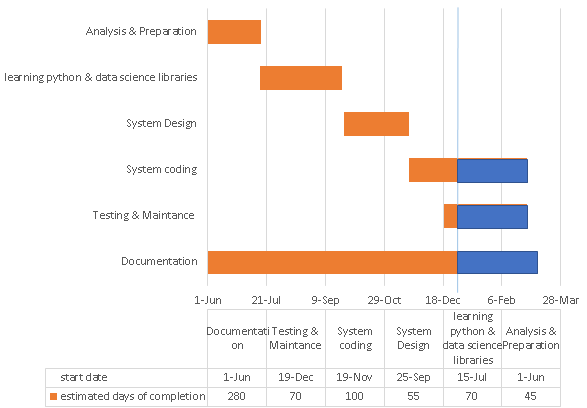
\includegraphics[scale=2]{Untitled.png} 
	\caption{Gantt chart} %figure name
	\label{Figure 1} % for referencing
\end{center}
\end{figure}
\chapter{Literature Review}
\section{Related Projects}
\subsection{Zillow}
It is a website in which people can buy houses, list houses to sell and the site gives an estimated data for the price of the house.
\subsection{Rentometer}
It is a website that uses proprietary technology and data to provide a thorough rent comparison analysis in seconds. By analysing recent rental listings in the surrounding neighbourhood, Rentometer can calculate rent prices based on location and apartment size, and provide a market rate estimate or lets the user know if he/she is paying too much rent.
\section{Related Research Works}
Anirudh Kaushal and Achyut Shankar researched in detail about house price prediction using multiple linear regression method. In the paper “House Price Prediction Using Multiple Linear Regression” published on April 25, 2021 there is explanation about filtering of data set, data processing, training and evaluating multiple linear regression model.[1]
Manasa, J., Gupta, R., \& Narahari, N.S. studied and compared the algorithms for estimation of price of houses in city of Bengaluru in the paper “Machine learning based predicting house prices using regression techniques”.[2]
\chapter{Methodology}

\subsection{Referring Section}
This is an example of referring Section \ref{sec:bkgrnd} of page \pageref{sec:bkgrnd}. Lorem ipsum dolor sit  amet, diam posidonium efficiantur pri ex, qui aliquip convenire an. Vim falli vivendum ei. Ei per congue sanctus pericula. Mei id tollit mentitum corrumpit. Ad paulo quaerendum eam, meis delenit concludaturque ea nec.\par
Sit id duis explicari, no pro quod nisl, erat nominati in his. Te choro efficiendi per. Vix alia munere an, ea aperiam expetenda ius. Id simul forensibus est, mei tacimates imperdiet incorrupte at, minim hendrerit ne per. Ex meliore verterem efficiendi vis.

Ea his munere torquatos, quidam essent luptatum cu pro. Ei duo scaevola electram. Vidit percipitur ut vim, ne his solet prodesset inciderint. Cum facilisi sententiae at, vis noster electram contentiones cu. Nec at eius novum diceret.

Lorem ipsum dolor sit  amet, diam posidonium efficiantur pri ex, qui aliquip convenire an. Vim falli vivendum ei. Ei per congue sanctus pericula. Mei id tollit mentitum corrumpit. Ad paulo quaerendum eam, meis delenit concludaturque ea nec.\par
Sit id duis explicari, no pro quod nisl, erat nominati in his. Te choro efficiendi per. Vix alia munere an, ea aperiam expetenda ius. Id simul forensibus est, mei tacimates imperdiet incorrupte at, minim hendrerit ne per. Ex meliore verterem efficiendi vis.

Ea his munere torquatos, quidam essent luptatum cu pro. Ei duo scaevola electram. Vidit percipitur ut vim, ne his solet prodesset inciderint. Cum facilisi sententiae at, vis noster electram contentiones cu. Nec at eius novum diceret.
\chapter{Figures and Tables}
\section{Section for Sample Figure}
Partem graece mucius est ei, usu ex facilisis dissentiet, probo prodesset scriptorem ius ea. Ne mei essent splendide, case tritani duo ei. Eam ne stet feugiat albucius. Ne diam dicant viderer eam, at pri minim vivendo periculis, in vix commodo invidunt. In eum omnis vocent aperiam. Sit prima atqui splendide ad, singulis recusabo quaerendum at his, enim eligendi forensibus ea eam.

Sed veri aeque persecuti ut. Ut accusam mediocrem accusamus eos, quis clita probatus ex his. Mea oratio deleniti interesset at. Odio melius antiopam eu his, ut nec tantas maiestatis ullamcorper. Ut numquam reprimique cum.

\begin{figure}[tbh] % tbh means top, bottom or here (priority: left to right)
\begin{center}
	\includegraphics[width = 3in]{images/sampleImage1.jpg}
	\caption{The Sample Image One} %figure name
	\label{figSample1} % for referencing
\end{center}
\end{figure}

\subsection{Referring Figure}
This is an example where Figure \ref{figSample1} of page \pageref{figSample1} is referenced. Detracto suavitate id per, no est putent accusata quaestio, purto quaeque oporteat ei sea. Id eam erat affert, ex has summo inimicus partiendo. Option aliquam imperdiet ius ex. Efficiendi omittantur in mea, id usu tacimates rationibus. Ei accusamus dissentias vix, eos aperiam percipit id.

Mea cu vitae noluisse. Tation eirmod iracundia sea no, duo no aliquando elaboraret. Qui ut legere mucius, dolore efficiendi definitionem quo ex. Usu te falli similique posidonium, eum eu dicat aeterno phaedrum, te paulo deleniti ius. Pro te aliquam platonem, eos ea dolore phaedrum. Graece honestatis sit at, nec id ubique legendos.

\section{Section for Sample Table}
Prompta albucius ne vel. Has te intellegat definitionem, vim duis animal adipiscing ei. At qui iisque accusata, id his possim nominati. Ne agam dissentias eos, dico vivendo percipit ut mea.

\begin{table}[tbh]
\centering
\caption{Table Example}
\begin{tabular}{|c|r|c|l|c|c|} %c,l,r represent alignment, number of c,l or r represent number of columns, | for Vertical line
	\hline %horizontal line
	x &3 &4 &5 &5 &5\\
	\hline %horizontal line
	f(x) &111 &22 &30 &40 &500\\
	\hline %horizontal line
\end{tabular}
\label{tblSampleTable}
\end{table}

\subsection{Referring Table}
This is an example where Table \ref{tblSampleTable} of page \pageref{tblSampleTable} is referenced. Detracto suavitate id per, no est putent accusata quaestio, purto quaeque oporteat ei sea. Id eam erat affert, ex has summo inimicus partiendo. Option aliquam imperdiet ius ex. Efficiendi omittantur in mea, id usu tacimates rationibus. Ei accusamus dissentias vix, eos aperiam percipit id.

Mea cu vitae noluisse. Tation eirmod iracundia sea no, duo no aliquando elaboraret. Qui ut legere mucius, dolore efficiendi definitionem quo ex. Usu te falli similique posidonium, eum eu dicat aeterno phaedrum, te paulo deleniti ius. Pro te aliquam platonem, eos ea dolore phaedrum. Graece honestatis sit at, nec id ubique legendos.
Detracto suavitate id per, no est putent accusata quaestio, purto quaeque oporteat ei sea. Id eam erat affert, ex has summo inimicus partiendo. Option aliquam imperdiet ius ex. Efficiendi omittantur in mea, id usu tacimates rationibus. Ei accusamus dissentias vix, eos aperiam percipit id.

Mea cu vitae noluisse. Tation eirmod iracundia sea no, duo no aliquando elaboraret. Qui ut legere mucius, dolore efficiendi definitionem quo ex. Usu te falli similique posidonium, eum eu dicat aeterno phaedrum, te paulo deleniti ius. Pro te aliquam platonem, eos ea dolore phaedrum. Graece honestatis sit at, nec id ubique legendos.
Detracto suavitate id per, no est putent accusata quaestio, purto quaeque oporteat ei sea. Id eam erat affert, ex has summo inimicus partiendo. Option aliquam imperdiet ius ex. Efficiendi omittantur in mea, id usu tacimates rationibus. Ei accusamus dissentias vix, eos aperiam percipit id.

Mea cu vitae noluisse. Tation eirmod iracundia sea no, duo no aliquando elaboraret. Qui ut legere mucius, dolore efficiendi definitionem quo ex. Usu te falli similique posidonium, eum eu dicat aeterno phaedrum, te paulo deleniti ius. Pro te aliquam platonem, eos ea dolore phaedrum. Graece honestatis sit at, nec id ubique legendos.
Detracto suavitate id per, no est putent accusata quaestio, purto quaeque oporteat ei sea. Id eam erat affert, ex has summo inimicus partiendo. Option aliquam imperdiet ius ex. Efficiendi omittantur in mea, id usu tacimates rationibus. Ei accusamus dissentias vix, eos aperiam percipit id.

Mea cu vitae noluisse. Tation eirmod iracundia sea no, duo no aliquando elaboraret. Qui ut legere mucius, dolore efficiendi definitionem quo ex. Usu te falli similique posidonium, eum eu dicat aeterno phaedrum, te paulo deleniti ius. Pro te aliquam platonem, eos ea dolore phaedrum. Graece honestatis sit at, nec id ubique legendos.

\section{Complex Table from Excel}
Complex tables can be created in MS-Excel and latex code for the table can be generated using "excel2latex" add-in.  An example of a complex table is shown in Table \ref{tab:complexTable} in page \pageref{tab:complexTable}\\ you can download excel2latex add-in from\\ 
https://www.ctan.org/tex-archive/support/excel2latex\\
Some extra packages are required. like bigstrut, multirow etc.
% Table generated by Excel2LaTeX from sheet 'Sheet1'
\begin{table}[htbp]
  \centering
  \caption{Complex table converted from Excel using excel2latex}
    \begin{tabular}{|c|c|c|c|c|c|}
    \hline
    SN    & Col 1 & Col 2 & \multicolumn{2}{c|}{Col 3} & Col 4 \bigstrut\\
    \hline
    1     & \multicolumn{2}{c|}{\multirow{2}[4]{*}{Merged Cells 1}} & a     & b     & e \bigstrut\\
\cline{1-1}\cline{4-6}    2     & \multicolumn{2}{c|}{} & c     & d     & \multirow{3}[6]{*}{f} \bigstrut\\
\cline{1-5}    3     & \multicolumn{4}{c|}{Merged Cells 2} &  \bigstrut\\
\cline{1-5}    \multirow{3}[6]{*}{4} & \multirow{3}[6]{*}{abc} & \multirow{5}[10]{*}{Merged Cells 3} & a1    & a2    &  \bigstrut\\
\cline{4-6}          &       &       & a3    & q     & ww \bigstrut\\
\cline{4-6}          &       &       & \multicolumn{2}{c|}{\multirow{2}[4]{*}{a4}} & as \bigstrut\\
\cline{1-2}\cline{6-6}    \multirow{2}[4]{*}{5} & a11   &       & \multicolumn{2}{c|}{} & qq \bigstrut\\
\cline{2-2}\cline{4-6}          &       &       & \multicolumn{3}{c|}{Merged} \bigstrut\\
    \hline
    \end{tabular}%
  \label{tab:complexTable}%
\end{table}%
Mea cu vitae noluisse. Tation eirmod iracundia sea no, duo no aliquando elaboraret. Qui ut legere mucius, dolore efficiendi definitionem quo ex. Usu te falli similique posidonium, eum eu dicat aeterno phaedrum, te paulo deleniti ius. Pro te aliquam platonem, eos ea dolore phaedrum. Graece honestatis sit at, nec id ubique legendos.
Detracto suavitate id per, no est putent accusata quaestio, purto quaeque oporteat ei sea. Id eam erat affert, ex has summo inimicus partiendo. Option aliquam imperdiet ius ex. Efficiendi omittantur in mea, id usu tacimates rationibus. Ei accusamus dissentias vix, eos aperiam percipit id.

Mea cu vitae noluisse. Tation eirmod iracundia sea no, duo no aliquando elaboraret. Qui ut legere mucius, dolore efficiendi definitionem quo ex. Usu te falli similique posidonium, eum eu dicat aeterno phaedrum, te paulo deleniti ius. Pro te aliquam platonem, eos ea dolore phaedrum. Graece honestatis sit at, nec id ubique legendos.
Detracto suavitate id per, no est putent accusata quaestio, purto quaeque oporteat ei sea. Id eam erat affert, ex has summo inimicus partiendo. Option aliquam imperdiet ius ex. Efficiendi omittantur in mea, id usu tacimates rationibus. Ei accusamus dissentias vix, eos aperiam percipit id.

Mea cu vitae noluisse. Tation eirmod iracundia sea no, duo no aliquando elaboraret. Qui ut legere mucius, dolore efficiendi definitionem quo ex. Usu te falli similique posidonium, eum eu dicat aeterno phaedrum, te paulo deleniti ius. Pro te aliquam platonem, eos ea dolore phaedrum. Graece honestatis sit at, nec id ubique legendos.
 
\chapter{Equations}

\section{Basics of Equations}
Mathematical expression within text can be written as $ y=mx+c $. In separate line as $$ ax + by + c = 0 $$
Some latex mathmatics examples:\\
Superscript:\\
$x^3$
$$x^3$$
$$x^{3x+4}$$
$$x^{{{3x+4}^4}+5}$$
Subscript:
$$x_{13}$$
${x_1}_2$
$${{{x_1}_2}_3}$$
Greek letters
$$\pi$$
$$\alpha$$
$\alpha A$
$\beta$
$\beta B$
$\delta$
$\gamma$
$\vartheta$
$\Theta$
$\phi$
$\varphi$
$\Phi$ 
trigonometric:
$y=\sin(\pi)$
Log:
$y=\log(\pi)$
$y=\ln(\pi)$
$y=\log_{10}$
Square root:
$\sqrt{2}$
$\sqrt[3]{4}$
$\sqrt{x^2+y^2}$
$\sqrt[3]{x^2+y^2}$
$\sqrt{\sqrt[3]{x^2+y^2}}$
Fraction:
About 2/3 of the class is full.
About $\frac{2}{3}$ of the class is full.
About $\displaystyle{\frac{2}{3}}$ of the class is full.
About $\displaystyle{\frac{\sqrt{\sqrt[3]{x^2+y^2}}}{\sqrt{x^2+x+1}}}$ of 
About $\displaystyle{\frac{2}{1+\sqrt{\sqrt[3]{x^2+y^2}}}}$ of the class is full.

Reserved characters:
$\{a,b,c\}$
\$20
$10\% of 100 is 100$
$10\,\,\,\% \;\;\; of \,\,\,100 \quad\qquad is\:\:\: 100$


Braket Style:
$3(\frac{2}{3})$
$3\left(Hello(\frac{2}{3})\right)$
$3\left\{Hello(\frac{2}{3})\right\}$
$3\left\{Hello(\frac{2}{3})\right.$
$3\left.Hello(\frac{2}{3})\right.$
$\left.\frac{dy}{dx}\right|_{x=1}$
( \big (  \Big (  \Bigg( 
$3(\frac{2}{3})$
$3\Big(\frac{2}{3}\Big)$

Equation:
\begin{equation} % for equations with equation numbers
% no need use $ sign
E=mc^2 
\end{equation}

\begin{equation*}
% no need use $ sign
E=mc^2 
\end{equation*}

\[
E=mc^2
\]

\begin{eqnarray}
E=mc^2 \label{eqn:mc2} \\ %labels are useful for referencing
E=mc^4\\
E=mc^7 
\end{eqnarray}

\begin{eqnarray*}
E=mc^2 \\
E=mc^4\\
E \approx \pm (mc^7 +3)\\
E \approx \pm (mc^7 +3)
\end{eqnarray*}
\begin{eqnarray}
E &=& mc^2 \\
E &=& mc^4 \nonumber \\
E &\approx& \pm (mc^7 +3)
\end{eqnarray}
Limit:
$\lim \limits_{x \to a} f(x)$\\
$\lim \limits_{x \to a} \frac{f(x)-f(a)}{x-a}=f'(a)$
Integration:
$\int$\\
$\int(\quad sin\quad x\quad dx= ) $\\
$\displaystyle{\int(\quad sin\quad x\quad dx= )} $
$\displaystyle{\int^b_a(\quad sin\quad x\quad dx= )} $
$\displaystyle{\int^b_a\: x^2\: dx\:=\left[\frac{x^3}{3}\right]^b_a} $
%$\displaystyle{\iiint^b_a\: x^2\: dx\: dy \: dz \:=\lim \limits_{x \to a}\left[\frac{x^3}{3}\right]^b_a} $


Summation:
$\displaystyle{\sum_{n=1}^{10}}$
$\displaystyle{\int^b_a\: f(x)\: dx\:=\lim \limits_{x \to \infty}\displaystyle{\sum_{K=1}^{10}f(x_k).\delta x}} $

\section{Referencing the Equation}
The Equation can be referenced using labels. example Equation \ref{eqn:mc2} of page \pageref{eqn:mc2} is referenced here.
LaTeX is the de facto standard for the communication and publication of scientific documents. LaTeX is available as free software.

\chapter{Listing Examples}
Here are some examples of listing\\
\textbf{Ordered List Technique:}\\
Listing Technique 1:
\vspace{-18pt} %use \vspace{-18pt} before list to reduce paragraph spacing between list and preceeding paragraph. 
\begin{enumerate}
\item Pencil
\item Paper
\item Calculator
\item Notebook
	\begin{enumerate}
	\item Assignment
		\begin{enumerate}
		\item Test
			\begin{enumerate}
			\item Test 1
			\item Test 2
			\end{enumerate}
		\item Quiz
		\end{enumerate}
	\item Classwork
	\end{enumerate}
\end{enumerate}

Listing Technique 2:
\vspace{-18pt}
\begin{itemize}
\item Pencil
\item Paper
\item Calculator
\item Notebook
	\begin{itemize}
		\item Assignment
		\begin{enumerate}
		\item Test
			\begin{itemize}
			\item Test 1
			\item Test 2
			\end{itemize}
		\item Quiz
		\end{enumerate}
	\item Classwork
	\end{itemize}
\end{itemize}

Listing Technique 3:
\vspace{-18pt}
\renewcommand{\labelenumii}{\Alph{enumii}}
\renewcommand{\labelenumiii}{\Roman{enumiii}}
\renewcommand{\labelenumiv}{\roman{enumiv}}
\begin{enumerate}
\item Pencil
\item Paper
\item Calculator
\item Notebook
	\begin{enumerate}
	\item Assignment
		\begin{enumerate}
		\item Test
			\begin{enumerate}
			\item Test 1
			\item Test 2
			\end{enumerate}
		\item Quiz
		\end{enumerate}
	\item Classwork
	\end{enumerate}
\end{enumerate}

\section{The Subsections}

LaTeX  is a document preparation system for the communication and publication of scientific documents. \par It is most often used for medium-to-large technical or scientific documents but it can be used for almost any form of publishing.
as said in \ref{sec:bkgrnd} of page no. \pageref{sec:bkgrnd}
LaTeX is the de facto standard for the communication and publication of scientific documents. LaTeX is available as free software.

\subsubsection{The subsubsection}
LaTeX  is a document preparation system for the communication and publication of scientific documents. \par It is most often used for medium-to-large technical or scientific documents but it can be used for almost any form of publishing.

LaTeX is the de facto standard for the communication and publication of scientific documents. LaTeX is available as free software.

\paragraph{The paragraph}
\ LaTeX  is a document preparation system for the communication and publication of scientific documents. \par It is most often used for medium-to-large technical or scientific documents but it can be used for almost any form of publishing.
\subparagraph{The subparagraph}
\ LaTeX  is a document preparation system for the communication and publication of scientific documents. \par It is most often used for medium-to-large technical or scientific documents but it can be used for almost any form of publishing.

 
\chapter{Citation Example}
\section{Citation and compiling bib file}
This is an example of citing texts \cite{Li2014}. This is second citation \cite{Yasir2014} The first cited reference will be numbered "1", second "2" and so on. Only those cited in the document will be listed in the reference section.

Note that to compile documents with reference correctly, you need to follow following steps:
\vspace{-18pt}
\begin{enumerate}
	\item Run pdfLatex (or Quick build)
	\item Run Bibtex 
	\item Run pdflatex 2 times
\end{enumerate}
 
Tation eirmod iracundia sea no, duo no aliquando elaboraret. Qui ut legere mucius, dolore efficiendi definitionem quo ex. Usu te falli similique posidonium, eum eu dicat aeterno phaedrum, te paulo deleniti ius. Pro te aliquam platonem, eos ea dolore phaedrum. Graece honestatis sit at, nec id ubique legendos.
Detracto suavitate id per, no est putent accusata quaestio, purto quaeque oporteat ei sea. Id eam erat affert, ex has summo inimicus partiendo. Option aliquam imperdiet ius ex. Efficiendi omittantur in mea, id usu tacimates rationibus. Ei accusamus dissentias vix, eos aperiam percipit id.

Mea cu vitae noluisse. Tation eirmod iracundia sea no, duo no aliquando elaboraret. Qui ut legere mucius, dolore efficiendi definitionem quo ex. Usu te falli similique posidonium, eum eu dicat aeterno phaedrum, te paulo deleniti ius. Pro te aliquam platonem, eos ea dolore phaedrum. Graece honestatis sit at, nec id ubique legendos.
Detracto suavitate id per, no est putent accusata quaestio, purto quaeque oporteat ei sea. Id eam erat affert, ex has summo inimicus partiendo. Option aliquam imperdiet ius ex. Efficiendi omittantur in mea, id usu tacimates rationibus. Ei accusamus dissentias vix, eos aperiam percipit id.

%Reference
\renewcommand\bibname{References} % Change heading to References
\bibliographystyle{IEEEtran} % to use IEEE Format for referencing
\addcontentsline{toc}{chapter}{References} % to add references in TOC
\bibliography{library} % specify the .bib file containing reference information 

%Comment this Chapter if you do not need to include Appendix.
\chapter*{Appendix}
\addcontentsline{toc}{chapter}{Appendix}
Appendix Text Comes Here

\end{document}
